\chapter{\sffamily Interacting with systems in general}

{\bfseries\sffamily Concept.} To design and build a software which can interact with stochastic processes of any kind, either manually through user input, or automatically by introducing a `policy'. The mathematical formalism and software that we introduce here will serve as a common language and interface for any simulation studies into manipulating real world phenomena, and will enable the learning of control algorithms in later chapters of this book. We will implement this new interaction software as an extension to the stochadex package. For the mathematically-inclined, this chapter will cover how interactions are structured in theory by adding some new concepts to the stochadex formalism and illustrating with some simple examples. For the programmers, the public Git repository for the code described in this chapter can be found here: \href{https://github.com/umbralcalc/stochadex}{https://github.com/umbralcalc/stochadex}.

\section{\sffamily Formalising general interactions}

Let's start by considering how we might adapt the mathematical formalism we have been using so far to be able to take actions which can manipulate the state at each timestep. Using the mathematical notation that we inherited from the stochadex, we may extend the formula for updating the state history matrix $X_{0:{\sf t}}\rightarrow X_{0:{\sf t}+1}$ to include a new layer of possible interactions which is facilitated by a new vector-valued `take action' function $G_{{\sf t}}$. In doing so we shall be defining the domain of an acting entity in the stochastic process environment --- which we shall hereafter refer to as simply the `agent'.

During a timestep over which actions are performed by the agent, the stochadex state update formula can be extended to include interactions by composition with the original state update function like so
%%
\begin{align}
X_{{\sf t}+1}^i &= G^i_{{\sf t}+1}[F_{{\sf t}+1}(X_{0:{\sf t}}, z, {\sf t}), A_{{\sf t}+1}] = {\cal F}^i_{{\sf t}+1}(X_{0:{\sf t}}, z, A_{{\sf t}+1}, {\sf t}) \label{eq:generalised-state-actions} \,,
\end{align}
%%
where we have also introduced the concept of the `actions' performed $A_{{\sf t}+1}$ on the system; some vector of parameters which define what actions are taken at timestep ${\sf t}+1$. The code for the new iteration formula would look something like Fig.~\ref{fig:iterations-with-actions}.

\begin{figure}[h]
\centering
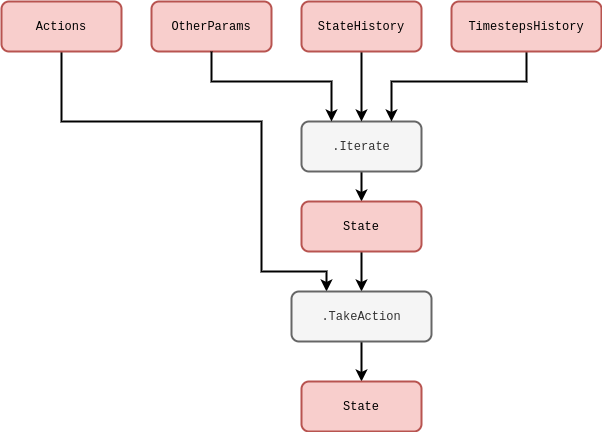
\includegraphics[width=11cm]{images/chapter-9-iterations-with-actions.drawio.png}
\caption{Code schematic of Eq.~(\ref{eq:generalised-state-actions}).}
\label{fig:iterations-with-actions}
\end{figure}

So far, Eq.~(\ref{eq:generalised-state-actions}) on its own will allow the agent to take actions that are scheduled up front through some fixed process or perhaps through user interaction via a game interface. So what's next? In order to start creating algorithms which will act on the system state for us, we need to develop a formalism which `closes the loop' by feeding information back from the stochastic process to the agent's decision-making algorithm.

If we use $A_{0:{\sf t}+1}$ a referring to the matrix of historically-taken actions which up to time ${\sf t}+1$, we can build up a more generalised, non-Markovian picture of automated interactions with the system which matches the notation we are already using for $X_{0:{\sf t}+1}$. Let us now define a Non-Markovian Decision Process (NMDP) as a probabilistic model which draws an actions matrix $A_{0:{\sf t}+1}=A$ from a `policy' distribution $\Pi_{({\sf t}+1){\sf t}}(A\vert X,\theta)$ given $X_{0:{\sf t}}=X$ and a new vector of parameters which fully specify the automated interations. Using the probabilistic notation from the previous part of the book, the joint probability that $X_{0:{\sf t}+1}=X$ and $A_{0:{\sf t}+1}=A$ at time ${\sf t}+1$ is
%%
\begin{align}
P_{{\sf t}+1}(X,A\vert z, \theta ) &= P_{{\sf t}}(X'\vert z,\theta ) \, \Pi_{({\sf t}+1){\sf t}}(A\vert X',\theta)P_{({\sf t}+1){\sf t}}(x\vert X',z,A) \label{eq:joint-prob-x-and-a} \,,
\end{align}
%%
where we recall that $P_{({\sf t}+1){\sf t}}(x\vert X',z,A)$ is the conditional probability of $X_{{\sf t}+1}=x$ given $X_{0:{\sf t}}=
X'$ and $z$ that we have encountered before, but it now requires $A_{0:{\sf t}+1}=A$ as another given input. We have illustrated Eq.~(\ref{eq:generalised-state-actions}) and how it relates to the policy distribution of Eq.~(\ref{eq:joint-prob-x-and-a}) with a new graph representation in Fig.~\ref{fig:fundamental-loop-with-actions}.

\begin{figure}[h]
\centering
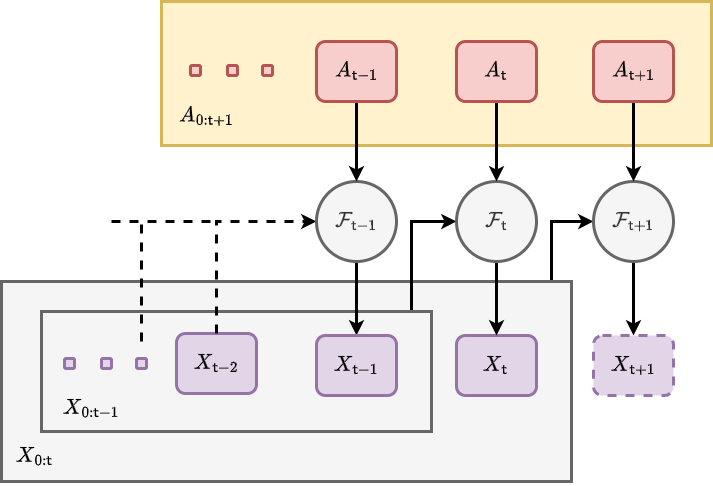
\includegraphics[width=11cm]{images/chapter-9-fundamental-loop-with-actions.drawio.png}
\caption{Graph representation of Eq.~(\ref{eq:generalised-state-actions}) with the policy distribution of Eq.~(\ref{eq:joint-prob-x-and-a}).}
\label{fig:fundamental-loop-with-actions}
\end{figure}

For additional clarity, let's take a moment to think about what $\Pi_{({\sf t}+1){\sf t}}(A\vert X,\theta)$ represents and how generally descriptive it can be. If an agent is acting under and entirely deterministic policy, then the policy distribution may be simplified to a direct function mapping which is parameterised by $\theta$. At the other extreme, the distribution may also describe a fully stochastic policy where actions are drawn randomly in time. If we combine this consideration of noise with the observation that policies described by a distribution $\Pi_{({\sf t}+1){\sf t}}(A\vert X,\theta)$ permit a memory of past actions and states, it's easy to see that this structure can be used in a wide variety of different use cases.

By marginalising over Eq.~(\ref{eq:joint-prob-x-and-a}) we find an updated probabilistic iteration formula for the stochastic process state which now takes the influence of agent actions into account
%%
\begin{align}
P_{{\sf t}+1}(X\vert z,\theta ) &= \int_{\Xi_{{\sf t}+1}}{\rm d}A \, P_{{\sf t}}(X'\vert z,\theta ) \, \Pi_{({\sf t}+1){\sf t}}(A\vert X',\theta)P_{({\sf t}+1){\sf t}}(x\vert X',z,A)  \,.
\end{align}
%%
This relationship will be very useful in the last part of this book when we begin to look at optimising control algorithms.

What are the main categories of action which are possible in the rows of $A$? Since the NMDP described by $\Pi_{({\sf t}+1){\sf t}}(A\vert X',\theta)$ is just another form of stochastic process, the main categories of action will fall into the same as those we covered in defining the stochadex formalism. The first, and perhaps most obvious, category would probably where the actions are defined in a continuous space and are continuously applied on every timestep. Some examples of these `continuously-acting' decision processes include controlling the temperature of chemical reactions~\cite{beeler2023chemgymrl} (such as those in a brewery), spacecraft control~\cite{tipaldi2022reinforcement} and guidance systems,  as well as the driving of autonomous vehicles~\cite{kiran2021deep}. Within a kind of subset of the continuously-acting category; we can also find the event-based acting decision processes (where actions are not necessarily taken every timestep), e.g. controlling traffic through signal timings~\cite{garg2018deep}, managing disease spread through treatment intervals~\cite{ohi2020exploring} and automated trading on stock markets~\cite{meng2019reinforcement}.

Many of the examples we have given above have continuous action spaces, but we might also consider classes of decision processes where actions are defined discretely. Examples of these include the famous multi-armed bandit problem~\cite{gittins2011multi} (like choosing between website layouts for E-commerce~\cite{liu2021map}), managing a sports team through player substitutions, sensor measurement scheduling~\cite{leong2020deep} and the sequential design prioritisation of large-scale scientific experiments~\cite{blau2022optimizing}.